\documentclass[10pt,twocolumn]{article}

% use the oxycomps style file
\usepackage{oxycomps}

% usage: \fixme[comments describing issue]{text to be fixed}
% define \fixme as not doing anything special
\newcommand{\fixme}[2][]{#2}
% overwrite it so it shows up as red
\renewcommand{\fixme}[2][]{\textcolor{red}{#2}}
% overwrite it again so related text shows as footnotes
%\renewcommand{\fixme}[2][]{\textcolor{red}{#2\footnote{#1}}}

% read references.bib for the bibtex data
\bibliography{references}

% include metadata in the generated pdf file
\pdfinfo{
    /Title (Computer Science Senior Comprehensive Project: \\A Web Interface for Angular Overlap Model Calculations)
    /Author (Jack Thomas-Colwell)
}

% set the title and author information
\title{Computer Science Senior Comprehensive Project: \\A Web Interface for Angular Overlap Model Calculations}
\author{Jack Thomas-Colwell}
\affiliation{Occidental College}
\email{jthomascolwe@oxy.edu}

\begin{document}

\maketitle
\newpage
\section{Introduction and Problem Context}
The properties and reactivity of any chemical system are fundamentally rooted in its unique electronic structure. In the simplest conceptualization, molecules are composed of atoms each of which contain electrons, protons, and neutrons. Over the past three centuries, this model of subatomic particles has undergone radical change from Dalton’s unary atom to Rutherford’s dense nucleus to modern quantum mechanical definitions. However, even though the Schrödinger equation first appeared almost a century ago, most people and media cling to the classical Bohr model of an electron orbiting a nucleus. While much easier to conceptualize, the circular orbits of classical mechanics fall woefully short in describing the complex quantum nature of electrons. Fundamentally, electrons are confined to discrete orbitals which describe their probability distribution about a nucleus. Within an atom, each of these orbitals will have a specific energy level which describes the stability of its occupying electron. Solving the Schrödinger equation, while tedious, gives rise to an exact analytical solution for these energy levels and the resulting electronic structure. However, this method quickly becomes impractical as the chemical system grows in complexity \cite{atkins2014}. Simply adding a second electron introduces enough complexity to make the Schrödinger equation fundamentally unsolvable. This analytical approach falls even further apart as one transitions from a single atom to a diatomic molecule. Given that most chemistry of interest involves complex molecules containing atoms upon atoms, there has been significant work over the past century to develop approximate methods to efficiently compute the electronic structures of molecules.

A particularly interesting subset of molecules are transition metal complexes. These molecules consist of a central transition-metal ion surrounded by a variety of bound molecules called ligands. Most atoms on the periodic table consist of electrons bound in s- and p-type orbitals. These orbitals are relatively simple in shape and have decently large energy gaps between them. Meanwhile, nearly all the transition metals have frontier electrons occupying d-type orbitals. These orbitals are much more complex in their shape and are very similar in energy. Unlike other orbitals, the energy gaps for d-type orbitals are on the same scale as electron-electron repulsion. This matched scale results in particularly intricate electronic structures and can lead to unique properties and reactivities; however, this significantly increases the difficulty of computing the electronic structures for transition metal complexes \cite{figgis2002}.

As it stands, there are two generally accepted computational approaches: density functional theory (DFT) and Ligand Field Theory. The first involves tasking a supercomputer with solving complex differential equations \cite{webmo}. After carefully inputting a molecule and letting the computation run, sometimes for days, the software will output the electronic structure. However, the nature of differential equations makes DFT functionally a black box. Short of repeating the long calculation with a new geometry or set of oxidation states, there is no way to intuitively understand the results. On the opposite end, Ligand Field Theory investigates orbital overlap integrals in search for a more analytical solution. While this theory does use transparent calculations and is very useful from an intuitive standpoint, its limitation lies in the scope of potential molecules. Due to the sheer complexity of a transition metal complex, analytical solutions are only accessible when one can use the molecular symmetry to simplify the problem. This limits Ligand Field Theory to molecules in idealized geometries such as an octahedron or a square plane \cite{larsen1974}.

The Angular Overlap Model (AOM) is a simplified version of Ligand Field Theory that vastly reduces the computational complexity and extends to model to all possible molecular geometries. This model leverages two key assumptions to simplify the problem. According to Ligand Field Theory, one must parameterize the orbital overlap integrals into their well-established Racah parameters A, B, and C to fully solve for the orbital energies in a transition metal complex. However, as previously discussed, some fundamental symmetry elements are required to make these calculations both feasible and meaningful \cite{underhill1966}. AOM instead abstracts all ligands into a set of two binding constants $e_\sigma$ and $e_\pi$. These parameters represent an optimal overlap where the central metal’s orbitals are perfectly aligned with the ligand. A fraction of this idealized overlap is then calculated based on the actual ligand position. Each ligand effect is then assumed to be additive resulting in an electronic structure after basic matrix addition \cite{larsen1974}. These assumptions greatly simplify the problem and allow for precise calculations for any possible geometry while maintaining transparency so that the process is intuitively accessible. While AOM does not deal with the multi-electron problem or configuration interactions, its predictions are still accurate for most complexes.

My project focuses on developing a webapp to make AOM calculations more accessible for both teaching and research purposes. While the computations used for AOM are leagues simpler than DFT or Ligand Field Theory, they still require a significant background in linear algebra to perform by hand. Conveniently enough, modern computers are incredibly well-suited to matrix algebra and can perform such calculations very efficiently. The main part of my project was the development of a calculator-type app that allows the user to input a range of molecules and compute their electronic structures. In addition to being of interest for computational chemists, AOM is incredibly useful as a teaching tool. Following a standard undergraduate chemistry curriculum, most students will take inorganic chemistry in the fall semester of their senior year during which they will learn about transition metals complexes in depth. However, the bonding and electronic properties of these complexes are fundamentally different than any other molecules that they will have encountered in previous coursework. General, organic, and physical chemistry all tend to focus on molecules with simpler ``standard'' bonding involving exclusively s- and p-type orbitals. Such bonding can, and often is, explained via the intuitive octet rule and valence bond theory. It is only when students begin studying transition metals that these approximate models are no longer sufficient. As such, many students must truly conceptualize how orbital overlap between a central metal ion and its ligands gives rise to the unique bonding properties of transition metal complexes. In my own experience as an inorganic chemistry student last year and in tutoring for the class this semester, I have found that this concept is truly the limiting step for understanding all of inorganic chemistry. AOM allows the user to see exactly how the positioning of a ligand can impact the bonding. To further amplify the model’s role as a teaching utility, the app contains a visualization tool that allows users to see both ligand positions and orbital shapes throughout the process. In addition to the calculator, the app also contains a page explaining exactly how AOM works and the underlying assumptions. There is also an accompanying problem set to guide students through both the app and specific facets of the model. All of these pieces together serve to tackle three main learning outcomes with the goal that students will be able to:
\begin{enumerate}
	\item understand how AOM calculations are performed and what assumptions are being made.
	\item conceptualize how specific ligands and ligand positions give rise to sigma and pi bonding in transition metal complexes.
	\item use AOM to generate quantitative splitting diagrams for transition metal complexes.
\end{enumerate}

\section{Technical Background}
% TODO

\section{Prior Work}
AOM has generally been neglected in the field of chemistry both in the literature and the pedagogy. The standard inorganic chemistry curriculum will spend weeks on crystal field theory and ligand field theory only to allocate a single lecture, if that, to AOM. Even then, most professors introduce AOM not as a computational model but rather as a list of points. The standard slide, an example of which is shown in Figure \ref{fig:aomslide}, lists off $e_\sigma$ and $e_\pi$ values for a select few possible ligand positions which can then be combined to give the standard octahedral, tetragonal, or square planar geometries with the more generous ones also allowing for a tetragonal bipyramidal structure. From there, students are given a few practice problems and never expected to touch the model again. This approach of teaching fundamentally mischaracterizes AOM as a computational tool. Showing that AOM is consistent with the predictions of Ligand Field Theory for the standard geometries is a great way to validate the model but neglects its true strengths. AOM is best suited for molecules of nonidealized geometries and should be taught as such by guiding students through the underlying computations and assumptions such that they can apply the model to novel molecular structures \cite{larsen1974}.

\begin{figure}
	\centering
	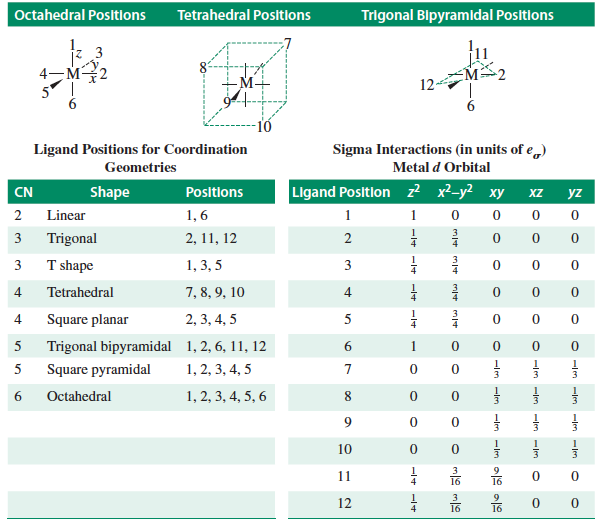
\includegraphics[width=.95\linewidth]{aomslide.png}
	\caption{
		A standard figure introducing AOM via a series of standard geometries \cite{miessler_inorganic_2014}.
	}
	\label{fig:aomslide}
\end{figure}

The inorganic chemistry course here at Occidental does a particularly good job with its introduction of AOM and was the original inspiration for this project. One of the problem sets given in this course asks students to use an old DOS program to compute various AOM matrices. Given that there is only one remaining computer in the chemistry department capable of running DOS, my chemistry advisor Dr. Michael Hill asked me to develop alternative software so that he could continue to give this problem set once that dinosaur of a computer eventually dies. Over the past year and a half, my chemistry research has focused on developing a computational package in Mathematica that uses AOM to investigate the particularly interesting electronic structure of bis(1,2-bis(diphenylphosphino)ethylene)cobalt(II). In studying this compound, I developed a Mathematica script capable of running AOM calculations for any given set of ligand positions \cite{thomascolwell2022}. However, this software was very specialized to the specific context of cobalt phosphine complexes and thus not particularly useful for teaching purposes. Moreover, Mathematica is a proprietary language and requires an expensive license to use further emphasizing the need for an accessible version of this software. 

This Mathematica script served as an initial reference for this project. In developing the webapp version of this software, I started by converting the computational package to Python so that I could serve it as a website. The old DOS software also provided valuable insight into my user interface design process. 

Outside of the old DOS software here at Occidental, an extensive review of computational and inorganic chemistry journals yielded exactly one other piece of software that uses AOM. In 2017, Bronova et. al. published a computational tool named ``BonnMag'' that computes the electronic structures of f-block elements \cite{bronova2018}. While a useful tool, their work does not cover the d-block transition metals in question. Rather than solely focusing on AOM, their model also employs advanced Ligand Field Theory calculations to supplement their results. This added complexity makes the software ill-suited for a webapp and requires a download and an installation. My project serves to uses a simpler model than that of BonnMag as to make the software more accessible and suitable for the web.

\section{Ethical Considerations}
While a piece of computational chemistry software may, at first glance, seem free of any ethical considerations, issues of inequitable access to computers and internet are still of great concern. As computers have become more and more prevalent in our society, those without reliable hardware or internet access become increasingly disadvantaged. Educational software is particularly dangerous as it is very easy to design curricula to use an online tool. Such tools can be a great aid to students; however, this can easily leave other students behind. Numerous studies have shown that this disparity in technological access, commonly called the digital divide, disproportionally affects underrepresented groups \cite{van2006}.

As one moves to higher levels of education, access to a computer and reliable internet becomes more normalized. Consequently, it grows easier to write off ethical concerns about access as irrelevant assuming that if each student is expected to type their papers, then they should be able to access any web-based tool they need. However, the technological requirements to write a paper can be very different that the requirements for a given piece of software, web or otherwise. Considering this, the general accessibility of a teaching tool is particularly important. Computationally expensive software often cannot run on weaker computers and leaves those students struggling for access. A key design principle in this project has been to minimize the front-end computations and therefore the technological requirements to run it. I have also tried to minimize the sheer quantity of data sent between the server and the client as to accommodate for weaker internet connections. Admittedly, any instructor using this project will need to guarantee student access. I fully plan to continue this project and confirm compatibility with various browsers and devices as to maximize accessibility. 

\section{Methods}
For this project, I developed a webapp capable of running AOM calculations for any given transition metal complex. The application also includes a series of teaching pages and problems aimed to familiarize students with AOM and transition metal bonding in general. The project was initially conceived as a single page webapp with the sole goal of allowing users to run AOM calculations in the browser. Through conversations with computer science professor Dr. Justin Li and inorganic chemistry professors Dr. Michael Hill and Dr. Bryan Hunter, I have worked to expand the idea to emphasize the teaching utility of this software. This aspect was highlighted through the aforementioned teaching pages and problem set. These pages serve to guide the student through AOM from a theoretical and practical perspective. The features of the calculator itself were also refined to best aid students in understanding the underlying bonding.

\subsection{Project Scope and Goals}
The AOM application is designed to be both a teaching and research tool with the emphasis placed on the former. From a computational chemistry perspective, the true strength of AOM lies in its ability to deal with non-idealized geometries in a very efficient manner. A computational package that allows researchers to compute these electron structures would be incredibly useful. That being said, most research projects are highly specialized to a given molecule or system. One such example is my prior work on cobalt(II) phosphine complexes from which this project stemmed. The Mathematica script for this paper needed to not only compute potential energy landscapes but to also minimize electronic transitions over more variables than a webapp can feasibly control. Given the incredibly large scope of potential molecules and chemical systems and the subsequent possible software requirements, I felt that this project would be much better suited towards teaching than research. From a teaching perspective, the ability to visualize how molecular geometry can impact the electronic structure is more than sufficient. It was much plausible to create a tool that can be used to help students understand transition metal bonding out of the box. Despite a heavy focus on its teaching utility, this project still provides a basis from which researchers could adapt the code to a given chemical system of interest. With this aim, the project has been thoroughly documented and all the functions that perform AOM calculation are contained in an isolated Python module for ease of extension.

As a teaching tool, AOM provides intuitively accessible calculations that other models such as DFT or Ligand Field Theory cannot. This intuition can be very useful to help students conceptualize how bonding works in transition metal complexes. Drawing on conversations with inorganic chemistry professors and my own experience in the course, I settled upon the following learning objectives. After using the app, a student should be able to:
\begin{enumerate}
	\item understand how AOM calculations are performed and what assumptions are being made.
	\item conceptualize how specific ligands and ligand positions give rise to sigma and pi bonding in transition metal complexes.
	\item use AOM to generate quantitative splitting diagrams for transition metal complexes.
\end{enumerate}

\subsection{Server Implementation}
This webapp is served via a Django webserver built entirely using Python. I originally intended to build this project without any underlying server which would have saved hosting costs. However, upon refining the project requirements, I settled upon using a back-end server.

Within an AOM calculation, each ligand is assigned values for $e_\sigma$ and $e_\pi$ bases on its intrinsic binding strengths. While unary values are more than sufficient to build a theoretical understanding of bonding, exact values are required to yield quantitative results. Moreover, having real-world values in the results allow students to better understand what they have computed. The electronic structures of transition metals complexes notoriously depend upon the electron pairing energy of around 15,000 wavenumbers being similar in magnitude to the orbital energy gaps. Without quantitative results, this tool could not emphasize this similarity in magnitude and would be insufficient to teach about inorganic complexes. The values of $e_\sigma$ and $e_\pi$ are relatively difficult to find in the literature. In my own research, my chemistry advisor and I were able to find only one paper that accurately lists these binding parameters for common ligands. Given this, it was important that users of the webapp be able to select these preset ligand values from a list rather than finding them on their own. While I could have hardcoded this list into the application, I felt that it was better to store it in a database for each of modification and expansion. This need for a database influenced me to use a back-end server.

As for the choice of backend framework, I chose Django based on its ease of use. Compared to NodeJS, Django works out of the box with minimal configuration \cite{django}. Given that the majority of AOM computations involve matrix algebra, NumPy was also a significant factor in my choice of Django over NodeJS. I have used NumPy for many projects in the past and was already very familiar with it prior to starting this project. Rather than find or develop a new linear algebra program, I decided to use Django as it is Python-based and compatible with NumPy. Along with all of this, I also wanted to learn Django. I have developed many projects in the past using NodeJS and simply wanted to learn another framework.
 
The main downside to using a backend server for my application was the deployment process. A serverless application can easily be deployed on GitHub Pages with a simple push \cite{githubpages}. On the other hand, using a back-end server requires hosting for both the Django server and the accompanying database. The deployment process can be relatively tedious and took a significant amount of time to complete \cite{deploying_django}. It also makes debugging the software more complicated as errors can occur both on the front-end and back-end. When starting this project, I chose Heroku as my hosting platform given that it had a free-tier and was relatively easy to deploy to; however, since then the service has discontinued this free version and requires monthly payments for both server and database hosting \cite{heroku_removal_of_free_tier}. As I continue this project, I intend to convert the app to be fully serverless to avoid these new costs and increase the projects longevity beyond what my wallet can support.

\subsection{Front-end Frameworks}
The front end is built almost entirely in vanilla JavaScript. Initially, I considered using a front-end framework such as React or VueJS; however, decided against it. These frameworks are great for complex applications with many reused components but are overkill for simple interfaces \cite{react}. For this project, most page components were used exactly once and did not require constant monitoring. It was easy enough to monitor for changes to the ligand inputs using a simple event listener. Given this, I decided that my project was not intricate enough in its UI to warrant a full-scale framework like React. This has allowed me to simplify the front-end code and minimize the number of packages that the user needs to load. 

To best aid students in conceptualizing metal ligand bonding, I implemented a visualization tool that shows the input molecule in real-time. As the user adds or changes ligands, this visualizer updates accordingly. The current ligand (in focus) is also highlighted to help orient students with the visualizer’s layout. For this tool, I initially tried to use WebGL for the 3D rendering as it was the most customizable option and does not require external libraries. However, I was quickly overwhelmed by the amount of work required to render a simple sphere and began to look for alternatives. Out of the possible options, D3JS and ThreeJS seemed to be the most popular and well maintained. I worked through the basic tutorials and documentations of each library and determined that D3JS was significantly more customizable and powerful; however, it required significantly more setup and minutia than ThreeJS \cite{threejs,d3} Given that my 3D models simply contained balls, sticks, and a few polygonal meshes, ThreeJS was more than sufficient for this project. I was able to build the visualizer using ThreeJS without hitting any of the library’s limitations making a point to abstract the visualizer into its own JavaScript module in case I needed to switch libraries at a later date. Since WebGL works at a very primitive level close to that of the graphics processing unit, it would have been much faster to run \cite{threejs_vs_webgl}. However, I was not rendering anything too complicated or computationally expensive. Within ThreeJS, I elected to use the least expensive materials and lighting models to improve performance \cite{threejs}.

Bonding in transition metal complexes occurs between the ligands and the d-orbitals on the central metal ion and is heavily dependent upon the physical overlap between these two. Compared to s- and p-type orbitals, the d-type orbitals have particularly complicated shapes, as show in Figure \ref{fig:dorbitals}, especially when expressed in a tetragonal basis set. Given this complexity, the webapp needed a way for students to visualize the d-orbital boundary surfaces while running their computations. I performed an extensive search of both Google and various chemistry journals and was unable to find equations for these boundary surfaces. This required that I compute them myself. Computing these surfaces requires integrating each one-electron wavefunction over all space to determine an equipotential boundary surface. Doing so, is very computationally expensive and does not yield nice equations. As such, I was unable to compute these on the front end. In leu of this, I wrote a Mathematica script to compute these surfaces and convert them to polygonal meshes so that I could render them in ThreeJS. This algorithm is detailed in \texttt{source/orbitals.nb} and simply integrates the wavefunction and solves for the boundary surface. This surface is then plotted and meshed using Mathematica’s built-in functions. While the script takes a significant amount of time to compile, it was easy to write given Mathematica’s symbolic nature. The output JSON file is then loaded into ThreeJS on the front-end as a 3D mesh. The user is then allowed to toggle each of the d-orbitals via a dropdown menu on the main page which can be seen in Figure \ref{fig:dorbitals-visualizer}.

\begin{figure}
	\centering
	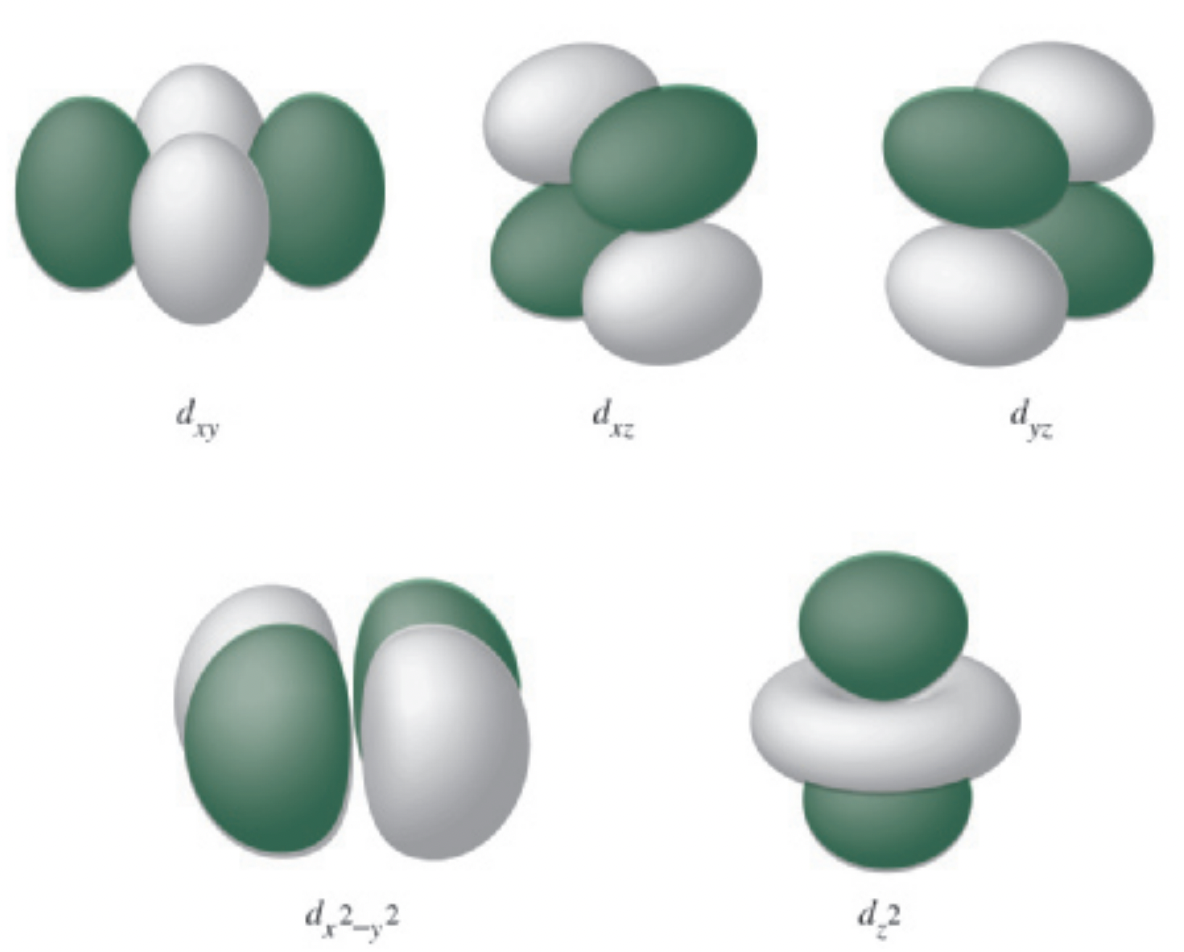
\includegraphics[width=.95\linewidth]{dorbitals.png}
	\caption{
		The five atomic d-type orbitals. \cite{miessler_inorganic_2014}.
	}
	\label{fig:dorbitals}
\end{figure}

\begin{figure}
	\centering
	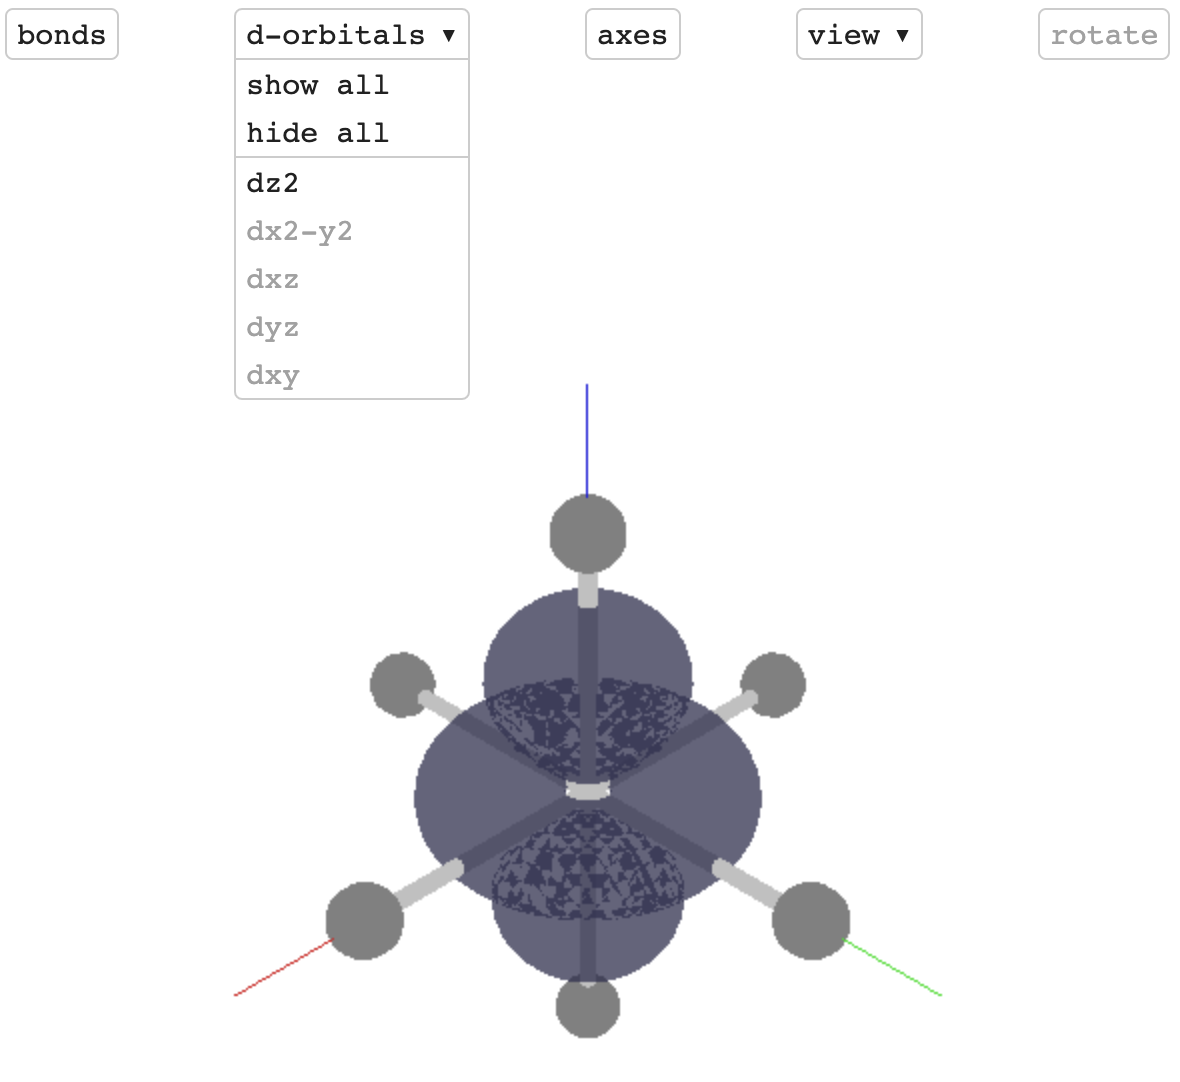
\includegraphics[width=.95\linewidth]{dorbitalsvisualizer.png}
	\caption{
		User interface to show the d-orbitals in the molecule visualizer.
	}
	\label{fig:dorbitals-visualizer}
\end{figure}

For the output plot, I decided to use ChartJS. Between the available libraries, it seemed that ChartJS and D3JS were the most popular. As with my decision about the visualizer, D3JS, while more customizable, required too much minutia to be useful for my project \cite{chartjs,d3,d3_vs_chartjs}. On the other hand, ChartJS was much easier implement and fit all my needs. I made a point to isolate the plot in its own JavaScript module in case I needed to switch libraries at a later date. 

\subsection{Interface Design}
The primary goal in designing the interface was to make it simple and intuitive. Rather than focus on making the page pretty, I opted to use a simple black and white color scheme. To highlight the inputs, I gave each field a label and underline which changed colors upon focus. Initially, I tried to use the default HTML5 input field but felt that it was too cluttered. To guarantee that the user inputs each coordinate for their ligands, I opted to use three discrete fields rather than allowing the user to enter an ordered pair. New ligands can be added via a button and preset values for $e_\sigma$ and $e_\pi$ can be selected using a dropdown. Throughout the design process, I consulted with inorganic chemistry professors to make sure that the design was intuitive. During each of these rounds of user testing, I did not give the professors any guidelines on how to use the app and simply watched them.

For the output page, the main goal was that users could visualize the change in their molecular geometry as they interacted with the plot. I accomplished this by updating the visualizer to the new geometry as the plot was hovered over. The AOM matrices and eigenvalues were also updated at this time. I considered having the metal-ligand distances change to reflect changes in $e_\sigma$ and $e_\pi$ but decided that this was counter-intuitive since it would imply that metal-ligand distances are relevant to AOM calculations which they are not. In the original DOS program, the user was able to toggle between sigma and pi effects. Rather than having separate pages, I decided to allow the user to simply toggle each effect with a button. This simplified the interface and allowed the user to visualize the various bonding types both individually and simultaneously.

A key feature in this project was the ability to share computations. Initially, I considered making a login system through which users could save and share their results; however, it was pointed out to me that this process could be greatly simplified by encoding the inputs into the URL. I chose to encode these inputs via a standard Base64 encoding in the URL fragment. While a natural language encoding would be much more intuitive and legible, the Base64 encoding significantly saves on space and disincentivizes the user from manually updating the URL fragment. It was necessary to use the fragment over the query string due to length limitations imposed by each browser. 

For the teaching pages, I tried to keep the interface as simple as possible. To make it easy to always return to the calculator, I opted to have the tutorial and problem set divided into discrete pages. Page navigation controls along with a button to return to the calculator are always shown at the bottom of the screen. The content of the teaching pages was adapted from an article by Erik Larsen and Gerd N. La Mar and serves to highlight how AOM works and what assumptions it makes. The problem set was written in collaboration with Dr. Michael Hill who is the inorganic chemistry professor here at Occidental. It served to highlight the same features of AOM and to address the learning outcomes which were listed earlier.

\section{Evaluation Metrics}
To formally evaluate my project, I focused on three main goals:
\begin{enumerate}
	\item Accuracy of the AOM calculations
	\item Ease of use of the webapp
	\item Success in teaching the learning outcomes
\end{enumerate}

These goals were evaluated in four general stages. The first served to validate the accuracy of the AOM calculations. To do this, I manually computed the AOM matrices for standard octahedral, square planar, and tetrahedral geometries and compared them with the results of the program. I also used the old DOS program to confirm that my on-paper calculations were accurate. The second involved ongoing conversations with two inorganic chemistry professors here at Occidental and at Northwestern University. These conversations served to guide my development process and minimize the number of changes that would be needed later on. The third stage was conducted after developing a working prototype of the calculator page. I met with each of the professors individually over Zoom and asked them to run calculations for standard and non-standard geometries. While they did this, I watched then go through the UI making note of any points of confusion. After they were done, I asked them explicitly to evaluate how intuitive the app was and if it would be useful in teaching students about inorganic bonding. The final round of user testing was conducted after the full app was functional including the calculator, teaching pages, and problem set. I repeated the same process as the previous stage with the inorganic professors. I also asked two students currently enrolled in inorganic chemistry to do the same evaluation process. They were ideal users as they had learned all of the prerequisite chemistry but had not yet been taught about AOM. 

\section{Results and Discussion}
\subsection{Calculation Accuracy Results}
As part of the first round, the program was evaluated against calculations done both by hand and by the old DOS program in the chemistry library. It was tested on octahedral, square planar, and tetragonal geometries. Each of these geometries were also rotated about the x, y, and z axes via a matrix transform to confirm that molecular orientation does not affect the orbital energies. The program was consistent with both standards on all geometries confirming that the calculations being performed are accurate.

\subsection{Ease of Use}
During the third round of evaluation, I observed two inorganic chemistry professors work through the calculator component of the software. Their interactions went as intended and they were able to input ligands and perform calculations as intended. However, they had significant trouble navigating between the start and end positions. At this point, I had it configures such that the ending ligand positions could only be entered once each of the starting positions had been submitted. One of the professors found this input to be very restrictive and unintuitive. He much preferred inputting one ligand at a time completing both the starting and ending states before moving to the next ligand. To fix this, I made it such that the end positions are auto-populated if and only if the starting positions have been fully entered. This design is consistent with when the ligand appears in the visualizer and is much more intuitive. It also prevents any weird cases where the auto-population would replace text entered by the user. Another problem arose with understanding the tool. My initial prototype lacked any text explanation short of the title ``Ligands''. Considering this feedback, I added a section of text at the top of both the input and results pages explaining what information was being shown and how to interact with it. When asked if the tool was intuitive, both professors said that it was short of the above problems. They also said that it would be very useful to teach students about bonding in transition metal complexes but would need instructions either in the app itself or during lecture.

Following the first round of user testing, I corrected the above problems and implemented the teaching pages. I then repeated the evaluation process in round four. This time, the professors had no trouble navigating the site and said that all of their previous concerns had been addressed. When asked to evaluate the application based on its design and teaching utility, both confirmed that the app was intuitive and would be useful as a teaching tool. To confirm that the newfound ease of use was not just a product of having used the application before, I proceeded to interview two students currently enrolled in inorganic chemistry. Both students had no trouble navigating the app and were able to correctly complete all the attached problems with minimal prompting. When asked how their knowledge of AOM and inorganic bonding mechanism had changed, both confirmed that the app improved their understanding. They found the visualization tool to be particularly useful in understanding how orbital overlap influenced bonding. 

\subsection{Conclusions and Next Steps}
Overall, I believe that the application met all of the intended goals. Evaluation results confirm that the calculations are accurate. After refining the app in response to user feedback, the interface is now intuitive and easy to navigate. User interviews confirm that the calculator and accompanying tutorial increased user understanding of AOM and inorganic bonding. Based on self-evaluation and their completion of the problem set, users were able to use the software to generate quantitative splitting diagrams as indented.

Given more time, I would have liked to interview more students about the utility of the app. Originally, I intended to interview the entire inorganic chemistry class here at Occidental; however, my prototype was not ready for user testing until November at which point all the students, myself included, were occupied with applications for graduate programs. More user testing would have been nice to truly confirm that the app is useful as a teaching tool in inorganic chemistry and to identify any faults. Self-evaluation is inherently subjective, and there is no clear-cut quantitative metric to measure understanding. These shortcomings can be corrected with a larger sample of users.

Admittedly, I have not thoroughly tested this software in browsers other that Google Chrome. Since Chrome is a widely used browser, this is not the most pressing issue; however, it would have been nice to present a project that is confirmed to work in all modern web browsers. I also did not optimize my application for mobile use. Given the complexity of the results and inputs, I decided that most users would be using this application from a computer rather than their phone. I asked each of my participants if mobile support were something that they would use, and most said that it would be nice but not a necessity. One key feature that users mentioned was tablet compatibility. As it stands, the app is not compatible with tablets, but I plan to modify it in the future to include this functionality.

Despite finishing senior seminar this semester, I fully plan to continue work on this project under the direction of my principal investigator Dr. Michael Hill. We intend to package this software with a PDF version of the accompanying problem set for publication in the Journal of Chemical Education.

\printbibliography

\end{document}
